\section{Event-based Deformation Control}\label{sec3}

To address the mentioned problem, the several potential force-based behaviors for each robot $i$ are used to synthetic to the proposed controller, which contains emergent strategies to navigate TVF to deal with the narrow space environment while ensuring the shape and the safety of TVF, named \textit{``Formation''}, and \textit{``Tailgating''}. In \textit{``Formation''} mode, the TVF maintains the original configuration, while in \textit{``Tailgating''} mode, the TVF transforms to the straight line configuration, as presented in Section~\ref{sec:config}. The detail of the proposed strategies is described in Fig.~\ref{fig:1control_diagram}.

\begin{figure*}
    \centering
    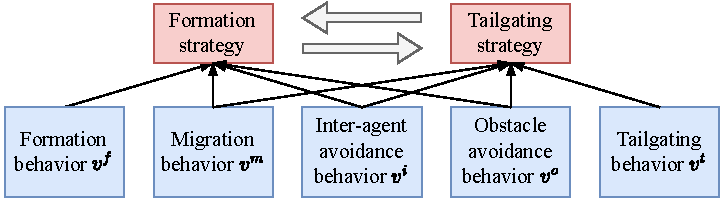
\includegraphics[width=0.65\textwidth]{paper2/images/control_diagram.pdf}
    \caption{Overview of the proposed event-based deformation control. The proposed strategy is constructed by two primary emergent strategy, including \textit{``Formation''} and \textit{``Tailgating''}, which are highlighted by red boxes. There are five individual behaviors that contribute to the emergent strategy, which illustrated via blue boxes.}
    \label{fig:1control_diagram}
\end{figure*}

\subsection{Individual behaviors}
According to~\cite{Vsrhelyi2018}, the potential field model is used to design individual behaviors a state-of-the-art model that allows robot swarm navigation in confined environments. From the original model, we design the rule of attraction for formation maintenance, tailgating and goal orientation; the rule of repulsion to prevent inter-robot collisions, and obstacle avoidance to avoid collisions with 
obstacles. 

Firstly, to ensure goal-directed motion in environments, a target reaching behavior is provided by a preferred velocity vector. We denote $v_\text{ref}$ is the preferred speed and $u_\text{ref}$ is the preferred direction~\cite{6095129}. Then, the migration term, equal for every agent, corresponds to:
\begin{equation}
    v_i^m=v_\text{ref}u_\text{ref}
\end{equation}

Secondly, the formation behavior is designed as an attractive force that drive robots to move toward their desired positions. Denote $\kappa\in\mathbb{R}$ be the scale ratio, which can be determined in Section~\ref{sec:edc}. Thus, a relative position-based controller of the form to maintain the desired shape, and enhance the abilities of TVF with scalable capabilities, which is given as follow:
\begin{equation}
    v^f_i=k_f\sum_{j=1}^n{\left(p_j-p_i-\kappa\left(\delta_j-\delta_i\right)\right)}
    \label{eqn:1uf}
\end{equation}
where $k_f>0$ is the formation control gain.

Next, the tailgating behavior is designed based on the relative position between each robot with other robot in the TVF, and used to navigate TVF pass through the narrow environment. Let robot $i$ follows robot ${l_i}$ within desired distance $d_\text{ref}$, with $d_\text{ref}>2r$,  an attractive force field for robot $i$ can be expressed as follows:
\begin{equation}
    v_i^t=\begin{cases}
k_t\left(p_{l_i}-p_i-d_\text{ref}\dfrac{v_{l_i}}{\left\Vert v_{l_i}\right\Vert}\right)+v_{l_i} & \text{if } l_i\neq-1\\
0 & \text{otherwise}
\end{cases}
    \label{eqn:1ut}
\end{equation}
where $k_t$ is the tailgating control gain. To determine the leader robot, the inner product $\tilde{p}_{ij}$ of the difference between robot $j$ in the neighbor set $\mathcal{N}_i$ with robot $i$, $p_j-p_i$, and the desired direction, $u_\text{ref}$, is given as follows:
\begin{equation}
    \tilde{p}_{ij} = \left\langle (p_j-p_i),u_\text{ref}\right\rangle
    \label{eqn:1tildep}
\end{equation}

As a result, the value of $\tilde{p}_{ij}$ is positive, proving that robot $j$ is in front of robot $i$ according to $u_\text{ref}$, and vice versa. For all robots $j$ in swarm, we obtain $\mathcal{P}_i=\left\{\tilde{p}_{ij}\right\}$. The leader robot ${l_i}$ of robot $i$ is chosen as the closest robot in front of it, i.e.
\begin{equation}
     l_i=\begin{cases}
    \arg\min_{j}\left\{\tilde{p}_{ij}\in\mathcal{P}_i\vert\tilde{p}_{ij}\geq0\right\} & \exists~\tilde{p}_{ij}\geq0\\ 
    -1 & \text{otherwise}
     \end{cases}
    \label{eqn:1li}
\end{equation}

Finally, inter-agent avoidance and obstacle avoidance behaviors are also designed to prevent collision. Denote $\mathcal{M}_i$ be the set of finite points on the obstacle's boundary, which are the closest to robot $i$, as illustrated in Fig.~\ref{fig:1model}. Those repulsive forces are given as follows:
\begin{equation}
    v_i^i=k_{i}\sum_{j=1,j\neq i}^n{v_{ij}^i}
\end{equation}
\begin{equation}
    v_i^o=k_o\sum_{o\in\mathcal{M}}v_{io}^o
\end{equation}
where $k_i,k_o>0$ is the inter-agent collision and obstacle avoidance gains, respectively. Denote $p_{ij}=p_i-p_j$, and $\hat{p}_{ij}=\dfrac{p_{ij}}{\left\Vert p_{ij}\right\Vert}$ be the relation position and the normalized vector between robot $i$ and robot $j$, respectively. Similarly, $p_{io}$, and $\hat{p}_{io}$ are the relative position and the normalized vector between robot $i$ and obstacle $o$, respectively, with $o\in\mathcal{M}_i$. Thus, the associated inter-agent avoidance $v_{ij}^i$ and obstacle avoidance $v_{io}^o$ are given as follows:
\begin{equation}
    v_{ij}^{i}=\begin{cases}
    \dfrac{r_a-\left\Vert p_{ij}\right\Vert}{r_a -2r}\hat{p}_{ij} & \text{if }\left\Vert p_{ij}\right\Vert<r_{a} \\
    0 & \text{otherwise}
    \end{cases}
    \label{eqn:1ui}
\end{equation}
\begin{equation}
    v_{io}^{o}=\begin{cases}
    \dfrac{r_a-\left\Vert p_{io}\right\Vert}{r_a -r}\hat{p}_{io} & \text{if }\left\Vert p_{io}\right\Vert<r_{a} \\
    0 & \text{otherwise}
    \end{cases}
    \label{eqn:1uo}
\end{equation}

\subsection{Event-based Deformation Control strategy}\label{sec:edc}

As mentioned in Fig.~\ref{fig:1control_diagram}, the proposed event-based deformation control includes two emergent strategies to navigate TVF safely through narrow space environment while maintaining the shape and ensuring the safety of swarm. At each time step, each robot determine the mode itself based on the sensing data collected from local sensor. The overall strategy can be summarised as follows:
\begin{equation}
    \tilde{v}_i=\begin{cases}
        v_i^f+v_i^m+v_i^c+v_i^o & \text{if mode = \textit{``Formation''}}\\
        v_i^t+v_i^m+v_i^c+v_i^o & \text{if mode = \textit{``Tailgating''}}
    \end{cases}
    \label{eqn:1v}
\end{equation}

To search the large parameter space $\mathcal{K}=\left\{k_f,k_t,k_i,k_o\right\}$ of the controller, evolutionary optimization can be used for highest-order flight and lowest number of collisions. The evaluation of the swarm behavior is based on a single fitness function that sums three independent values, including order, agent-safety, and obs-safety, smaller or equal to 1 (ideal case). The fitness is determined in simulations where the swarm is initialized with random positions in an environment where obstacles are  randomly placed. The description  to seek parameter values are similar and detailed in the~\cite{Vsrhelyi2018}.

To select the suitable mode at each time step, an event-based mode switching is designed to deal with the requirement to navigate a TVF through a narrow space environment. According to the individual behaviors and emergent strategies mentioned above, the mode of each robot can be changed based on its sense with environment around.

\begin{figure}
    \centering
    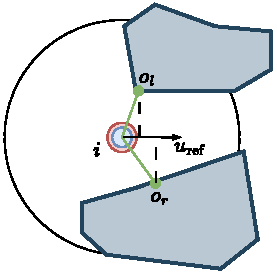
\includegraphics[width=0.35\textwidth]{paper2/images/we.pdf}
    \caption{Environment's width estimation}
    \label{fig:1we}
\end{figure}

Each obstacle point in the set $\mathcal{M}_{i}$ is clustered into two clusters on the left and right sides of the robot in $u_\text{ref}$ direction. Denote $o_l$ and $o_r$ respectively be the nearest obstacle point on the left and right sides whose distance to the robot $i$ is minimum. If $o_l$ and $o_r$ exist, the width of the environment can be estimated as follows:
\begin{equation}
    w_e= \left\vert\left\langle\left(o_r-o_l\right),u_\text{ref}\right\rangle\right\vert
    \label{eqn:1we}
\end{equation}

The estimation of the environment's width can be depicted in Fig.~\ref{fig:1we}. Besides, the formation's width $w_f$ can be easily determined through the predefined formation topology. Given the widths of the environment and formation, the scaling factor $\kappa$, which contributes to \eqref{eqn:1uf}, can be computed as follows:
\begin{equation}
    \kappa=\dfrac{w_e-2r}{w_f}
    \label{eqn:1kappa}
\end{equation}

As a result, each robot $i$ can choose its mode and compute scaling factor $\kappa$. Denote $\lambda>2$ be the threshold to transform between two mode. As presented in Algorithm~\ref{alg:1our}, the desired velocity $\tilde{v}_i$ corresponding to its mode can be obtained.
\begin{algorithm}[h!]
\caption{Pseudocode of the EDC strategy}
\label{alg:1our}
Get a set of observed obstacle points $\mathcal{M}_i$\;
\If{$\mathcal{M}_i$ is empty}{
    mode $\leftarrow$ \textit{``Formation''}\;
    $\kappa \leftarrow 1.0$\;
}
\Else{
    Determine the obstacle points $o_l$, $o_r$\;
    \If{$\nexists o_l$ or $\nexists o_r$}{
        mode $\leftarrow$ \textit{``Formation''}\;
        $\kappa \leftarrow 1.0$\;
    }
    \Else{
        Get the space's width $w_e$\tcc*[r]{Eq. \ref{eqn:1we}}
        \If{$w_e\leq\lambda r$}{
            mode $\leftarrow$ \textit{``Tailgating''}\;
        }
        \Else{
            mode $\leftarrow$ \textit{``Formation''}\;
            Estimate the desired formation width $w_f$\;
            \If{$w_e-2r\leq w_f$}{
                Compute the scaling factor $\kappa$\tcc*[r]{Eq. \ref{eqn:1kappa}}
            }
            \Else{
                $\kappa\leftarrow1.0$\;
            }
        }
    }
}
Compute desired velocity $\tilde{v}_i$\tcc*[r]{Eq. \ref{eqn:1v}}
\Return $\tilde{v}_i$\;
\end{algorithm}

After summing the contributions, we apply a cutoff on the acceleration at $u_\text{max}$ according to
\begin{equation}
    u_i=\dfrac{\tilde{u}_i}{\left\Vert\tilde{u}_i\right\Vert}\min(\left\Vert\tilde{u}_i\right\Vert, u_\text{max})
\end{equation}
where $\tilde{u}_i(k+1) =(\tilde{v}_i(k+1)-\tilde{v}_i(k)) /\tau$. Then, we apply a cutoff on the speed at $v_\text{max}$, and get the velocity command $v_i$ as follows:
\begin{equation}
    v_i=\dfrac{\tilde{v}_i}{\left\Vert\tilde{v}_i\right\Vert}\min(\left\Vert\tilde{v}_i\right\Vert, v_\text{max})
\end{equation}

\subsection{Stability analysis}
\begin{theorem}\label{the:stability}
Given the TVF as described in~\eqref{eqn:1model}, under the control law given in \eqref{eqn:1v}, the TVF asymptotically converges to the desired configuration.
\end{theorem}
\begin{proof}
To prove Theorem~\ref{the:stability}, we consider the negligible effect of collision avoidance behaviors and also neglect the constant impact of migration behavior, for any time $t(k)$, thus we conduct a stability analysis of the TVF in main contributions, i.e. formation and tailgating behaviors, which located in two separate modes, \textit{``Formation''} and \textit{``Tailgating''}, as mentioned in Section~\ref{sec:config}, which together ultimately lead to our conclusion.

\textbf{Mode \textit{``Formation''}:} Denote $L$ be the Laplacian matrix of the interaction topology graph of the swarm. Due to the fully connected, the entries of $L=\left[l_{ij}\right]$ are given as follows:
\begin{equation}
    l_{ij}=\begin{cases}
    -1 & \text{if }i\neq j \\
    n-1 & \text{if }i=j
    \end{cases}
\end{equation}

The control law \eqref{eqn:1uf} can be shown as follows:
\begin{equation}
    k_f\sum_{j=1}^n{\left(p_j-p_i-\kappa \delta_{ji}\right)}=k_f\sum_{j=1}^n{\left(p_j-p_i\right)}+b_i
\end{equation}
where the bias $b_i=-k_f\sum_{j=1}^n\kappa \delta_{ji}$.  In order to use the properties of the Laplacian matrix, the dynamics of the swarm system with the control law can be expressed as follows:
\begin{equation}
    \dot{P}=-k_fLP+B
\end{equation}
where $P=\left[p_1,...,p_n\right]^T$, $B=\left[b_1,...,b_n\right]^T$ and $L$ is the Laplacian matrix of the interaction topology graph of the formation. For these values of its elements the Laplacian matrix has only one zero eigenvalue and the rest of its eigenvalues are positive and the same. Note also that the vector $B$ is an eigenvector of $L$ with the corresponding eigenvalue $n$ and:
\begin{equation}
    LB=nB
\end{equation}

Defined the Lyapunov-like function for the TVF system as follows:
\begin{equation}
    V_f=\dfrac{1}{2}\left(P-\dfrac{1}{k_fn}B\right)^T\left(P-\dfrac{1}{k_fn}B\right)
\end{equation}

Talking the first derivative of $V_f$ gives
\begin{equation}
\begin{aligned}
    \dot{V}_f&=\left(P-\dfrac{1}{k_fn}B\right)^T\left(-k_fLP+B\right)\\
    &=-k_f\left(P-\dfrac{1}{k_fn}B\right)^TL\left(P-\dfrac{1}{k_fn}B\right)\leq0
\end{aligned}
\end{equation}

According to the LaSalle’s invariance
principle, it can be stated that as $k\to\infty$ the state $P$ will converge to the largest invariant subset $\Omega=\left\{P|\dot{V}_f=0\right\}$. In other words, the formation will close to the desired shape.

\textbf{Mode \textit{``Tailgating''}:} In case robot $i$ do not have it leader, we do not analysis the stability, because this robot do not contribute to the configuration maintenance of the TVF. Otherwise, in case robot $i$ has its leader $l_i$, we define a candidate Lyapunov function as follows:
\begin{equation}
    V_{t}=\dfrac{1}{2}\left(p_{l_i}-p_{i}-d_\text{ref}\dfrac{v_{l_i}}{\left\Vert v_{l_i}\right\Vert}\right)^{T}\left(p_{l_i}-p_{i}-d_\text{ref}\dfrac{v_{l_i}}{\left\Vert v_{l_i}\right\Vert}\right)
\end{equation}

Taking the first derivative of $V_t$, gives:
\begin{equation}
    \dot{V}_{t}=\left(p_{l_i}-p_{i}-d_\text{ref}\dfrac{v_{l_i}}{\left\Vert v_{l_i}\right\Vert}\right)^{T}\left(v_{l_i}-v_{i}\right)
\end{equation}

By using the control law $v^t_i$ in \eqref{eqn:1ut}, $\dot{V}_t$ becomes:
\begin{equation}
    \dot{V}_{t}=-k_{t}\left(p_{l_i}-p_{i}-d_\text{ref}\dfrac{v_{l_i}}{\left\Vert v_{l_i}\right\Vert}\right)^{T}\left(p_{l_i}-p_{i}-d_\text{ref}\dfrac{v_{l_i}}{\left\Vert v_{l_i}\right\Vert}\right)\leq0
\end{equation}

Therefore, the Lyapunov stability is satisfied. That leads to robot $i$ converges to its leader $l_i$ and keep behind a distance $d_\text{ref}$ along its leader direction. As a result, the straight line configuration can be guaranteed.
\end{proof}

\begin{remark}
In the research of this paper, decentralized control architecture is adopted for the TVF, i.e., each robot in the formation can decide the mode itself based on the information collected from surrounding environment. Correspondingly, the event-triggering condition we designed in Algorithm~\ref{alg:1our} is also distributed and presented in the form of compact sets. Besides, the control law \eqref{eqn:1v} is demonstrated stability based on Lyapunov theory. Under the action of the designed control law, the TVF will asymptotically achieve the desired configuration in both modes.
\end{remark}